
\section{Implementazione di una DNN}
Supponiamo di dover risolvere un problema di classificazione su un dataset di 
immagini. Le reti neurali profonde (DNN) descritte in precedenza possono 
essere utilizzate per risolvere questa tipologie di problema di classificazione.
Una possibile esempio applicativo consisterebbe nella classificazione 
di immagini del dataset MNIST.

MNIST è un famosissimo dataset di immagini di $28$x$28$ pixel in 
scala di grigio, in cui ogni immagine raffigura un numero intero 
$n \in \left\{0, 1, ..., 9\right\}$ scritto a mano.

\begin{figure}[H]
    \centering
    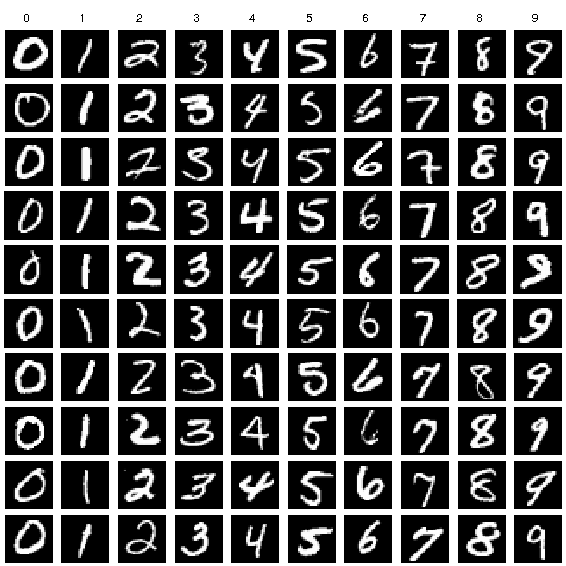
\includegraphics[width=0.5\textwidth]{Immagini/Generiche/MNIST_esempio.png}
    \caption{Esempio di immagini estratte dal dataset MNIST}
\end{figure}

Questo dataset possiede possiede $60000$ immagini training. E ha a 
disposizione un set di test composto da $10000$ immagini.

Un problema di classificazione sul dataset MNIST consisterebbe nel 
classificare correttamente l’immagine data in input restituendo in 
output il numero rappresentato dall'immagine.

Come visto un precedenza, le DNN usano come input un array 
(ovvero un vettore), mentre le immagini vengono rappresentate come
delle matrici. Pertanto, quando la rete neurale riceve in input un’immagine, 
essa viene interpretata come un array di pixel di $28 \cdot 28 = 784$ 
elementi.
Inoltre, nel dataset MNIST, ogni pixel dell'immagine assume un valore 
$\in[0, 255]$ a seconda dell’intensità del colore ad esso associato. 
Nella pratica, questo valore viene normalizzato nell'intervallo $[0, 1]$. 
Questa operazione di normalizzazione viene fatta per evitare che 
valori molto grandi generino gradienti sproporzionati durante la fase della
backpropagation, in quanto potrebbe causare instabilità numerica.
Essa permette anche di sfruttare più efficacemente le funzioni di 
attivazione, accelerare la convergenza e facilitare 
l'addestramento del modello.

\subsection{Implementazione}
Per risolvere il problema precedentemente descritto, una semplice 
rete neurale che potrebbe essere utilizzata per la classificazione 
delle imamgini potrebbe essere:

\begin{figure}[H]
    \centering
    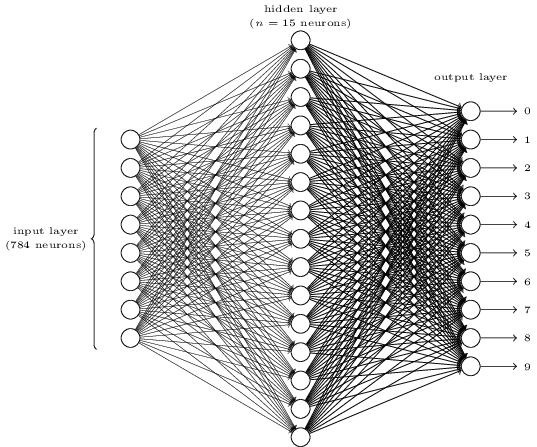
\includegraphics[width=0.9\textwidth]{Immagini/Grafici/DNN_MNIST.png}
    \caption{ Esempio di rete neurale fully connected utilizzata per risolvere un problema di
    classificazione sul dataset MNIST.}
    \label{fig:DNN_MNIST}
\end{figure}

Come si osserva, la rete possiede: $784$ neuroni di input, un hidden layer 
composto da 15 neuroni e un layer di output composto da 10 neuroni, uno 
per ogni classe.

Implementare a mano una rete del genere risulterebbe complicato, pertanto,
per implementare la rete e gestire la fase di training, ci affideremo al 
framework pytorch.
\\
La rete precedentemente descritta dalla figura (\ref{fig:DNN_MNIST}) 
può essere realizzata in python nel seguente modo:

\begin{lstlisting}
import torch.nn.functional as F
from torch import nn
import torch
from torch.utils.data import DataLoader, Dataset
from torchvision import datasets, transforms

class Network(nn.Module):
    def __init__(self, input_dim: int, hidden_dim: int, output_dim: int):
        super(Network, self).__init__()
        
        self._net = nn.Sequential (
            # Operazione di Flatten dell'immagine (28x28 -> 784)
            nn.Flatten(),                      
            
            # Input layer
            nn.Linear(input_dim, hidden_dim),  

            # Funzione di attivazione ReLU
            nn.ReLU(), 
            
            # Hidden layer
            nn.Linear(hidden_dim, output_dim), 
        )
        
    def forward(self, x: torch.tensor) -> torch.tensor:
        return self._net(x)
    
    def predict(self, x: torch.tensor) -> torch.tensor:
        return F.softmax(self._net(x), dim=1)

\end{lstlisting}

Come si può osservare, ogni qual volta bisogna creare una rete neurale o 
un sua componente, in pytorch, bisogna sempre creare una classe che 
estenda la classe \textit{nn.Module}, la quale fornisce tutte le funzioni di 
base per poter operare e interagire con le varie componenti del framework.
 
Inoltre, la funzione di attivazione softmax, non è stata utilizzata 
direttamente all'interno della rete, bensi all'esterno, in un altra funzione. Questo perchè, come poi si vedrà inseguito, verrà utilizzata 
come funzione di loss la \textit{cross-entropy}, la quale presenta già 
all'interno una specie di softmax. 

Il modello verrà poi instaziato con i seguenti parametri

\begin{lstlisting}
def main():

    device = torch.device("cuda" if torch.cuda.is_available() else "cpu")
    model = Network(784, 15, 10).to(device)
    ...
\end{lstlisting}

Il \textit{device} corrisponde al tipo di acceleratore (CPU, GPU, TPU, ...) 
per la rete neurale, ovvero dove verrà eseguita la rete neurale.
In questo caso, se la GPU è disponibile, la rete neurale verrà caricata nella 
VRAM della scheda video, permettono così di sfruttare la parelizzazione della
GPU accelerando i calcoli della rete neurale. 

Per quanto riguarda il dataset, pytorch fornisce già un'interfaccia per poterno
scaricare ed utilizzare, richiamabile nel seguente modo:

\begin{lstlisting}
    ...

    transform = transforms.Compose([
        transforms.ToTensor(),
    ])

    train_dataset = datasets.MNIST(root="\\tmp\\data", train=True, download=True, transform=transform)
    test_dataset = datasets.MNIST(root="\\tmp\\data", train=False, download=True, transform=transform)

    ...
\end{lstlisting}

Le \textit{transforms} vengono utilizzate per applicare delle "trasformazioni"
sui dati. Pytorch mette a disposizione moltissime tipologie di \textit{transforms} 
che possono essere utilizzati per diverse applicazioni.
In questo caso abbiamo soltanto utilizzato la trasformazione che converte l'immagine
in un tensore.


Successivamente dal dataset di test, selezioniamo una porzione da utilizzare come 
validazione del training. E definiamo i dataloader, ovvero i componenti che si 
occupano di prendere i dati dal dataset. 

Il dataloader permette anche di poter specificare la dimensione della batch (ovvero 
il numero di "campioni" da utilizzare per il calcole dei gradienti) ed il numero 
dei workers. Ogni worker corrisponde a un processo che viene assegnato 
a un core differente della CPU, permettendo così di parallelizzare il caricamento 
dei dati dal dataset. Tipicamente vengono utilizzati 4 worker per GPU. Tuttavia,
troppi worker attivi posso creare un'eccessivo overhead, rallentando così il sistema.

Un altro aspetto dei dataloader, è la possibilità di selezionare in modo randomico
gli elementi da prelevare, mettendo a "True" l'opzione \textit{shuffle}.

\begin{lstlisting}
    ...
    train_size = int(0.8 * len(train_dataset))
    val_size = len(train_dataset) - train_size
    train_subset, val_subset = torch.utils.data.random_split(train_dataset, [train_size, val_size])

    train_loader = DataLoader(dataset=train_subset, batch_size=64, shuffle=True, num_workers=4)
    val_loader = DataLoader(dataset=val_subset, batch_size=64, shuffle=False, num_workers=4)
    test_loader = DataLoader(dataset=test_dataset, batch_size=1, shuffle=False)
    ...
\end{lstlisting}


Per svolgere il training della rete neurale definiamo una funzione
che prenda come argomento: il tipo di acceleratore, il modello della 
rete neurale, il dataloader dei dati di training e di validation ed il numero 
di epoche.

Questa funzione, poi restituirà tutti i valori di loss e il valore 
dell'accuratezza di ogni epoca. Questi valori poi potranno essere utilizzati 
per visualizzare i risultati ottenuti dal training.  


\begin{lstlisting}

    def train(device, model: nn.Module, train_dataloader, valid_dataloader, epochs: int) -> Tuple[np.array, np.array, np.array]:
    
    criterion = nn.CrossEntropyLoss() 
    optimizer = torch.optim.Adam(model.parameters(), lr=1e-4)
    
    train_losses = np.zeros(epochs)
    valid_losses = np.zeros(epochs)
    val_accuracies = np.zeros(epochs)

    for epoch in range(epochs):
        
        epoch_losses_train: np.array = np.zeros(len(train_dataloader))
        epoch_losses_valid: np.array = np.zeros(len(valid_dataloader))
        
        #Fase di training
        model.train() 

        for batch_idx, (data, labels) in enumerate(train_dataloader):
            data, labels = data.to(device), labels.to(device)
            
            # Azzeramento dei gradienti
            optimizer.zero_grad() 
            # Forward              
            output = model(data) 
            # Calcolo della perdita               
            loss = criterion(output, labels)    
            
            # Backpropagation e aggiornamento dei pesi
            loss.backward()
            optimizer.step()

        
            epoch_losses_train[batch_idx] = loss.item()
        
        
        #Fase di validation
        model.eval()
        correct_val = 0
        total_val = 0
       
        with torch.no_grad():
            for batch_idx, (data, labels) in enumerate(valid_dataloader):
                data, labels = data.to(device), labels.to(device)

                output = model(data)
                loss = criterion(output, labels)
                epoch_losses_valid[batch_idx] = loss.item()
                
                # Calcolo accuratezza
                predictions = torch.argmax(output, dim=1)
                correct_val += (predictions == labels).sum().item()
                total_val += labels.size(0)
        
        
        #calcolo delle loss medie
        train_losses[epoch] = epoch_losses_train.sum() / len(train_dataloader)
        valid_losses[epoch] = epoch_losses_valid.sum() / len(valid_dataloader)
        val_accuracies[epoch] = correct_val / total_val
        
        print(f'Epoch [{epoch+1}/{epochs}], Training_Loss: {train_losses[epoch]:.6f}, Validation_Loss: {valid_losses[epoch]:.6f}, Accuracy: {val_accuracies[epoch]:.4f}"')
    
    return train_losses, valid_losses, val_accuracies
\end{lstlisting}

Mentre per valutare la precisione del modello su dati mai visti, definiamo la
funzione

\begin{lstlisting}
def test(device, model: nn.Module, test_loader: DataLoader) -> Tuple[np.array,np.array] :
    model.eval()
    all_preds = []
    all_labels = []

    with torch.no_grad():
        for data, labels in test_loader:
            data, labels = data.to(device), labels.to(device)
            output = model(data)
            predictions = torch.argmax(output, dim=1)

            all_preds.extend(predictions.cpu().numpy())
            all_labels.extend(labels.cpu().numpy())

    return np.array(all_labels), np.array(all_preds)
\end{lstlisting}

Questa funzione restituisce due liste dove, per un specifico indice $i$, la prima 
lista rappresenta il valore reale, mentre la seconda lista rappresenta il valore 
predetto dalla rete. 

\newpage
Per visualizzare dei campioni casuali dal dataset di test, definiamo la funzione 
\begin{lstlisting}
def display_random_test_sample(device, model: nn.Module, test_dataset):
    model.eval()
    indices = np.random.choice(len(test_dataset), size=64, replace=False)
    images, labels = zip(*[test_dataset[idx] for idx in indices])

    images = torch.stack(images).to(device)
    with torch.no_grad():
        probabilities = model.predict(images)
        predicted_classes = torch.argmax(probabilities, dim=1)

    fig, axes = plt.subplots(8, 8, figsize=(12, 12))
    for i, ax in enumerate(axes.flat):
        image = images[i].cpu().squeeze().numpy() * 255
        image = image.astype(np.uint8)

        ax.imshow(image, cmap='gray')
        true_label = labels[i]
        pred_label = predicted_classes[i].item()
        pred_prob = probabilities[i, pred_label].item()
        
        text1 = f"Predicted: {pred_label}"
        text2 = f"probability: {pred_prob:.3f}"

        if true_label == pred_label:
            ax.set_title(f"{text1}\n{text2}", fontsize=10, color="green")
        else:
            ax.set_title(f"{text1}\n{text2}", fontsize=10, color="red")
        ax.axis('off')
    ...
\end{lstlisting}


Infine, nella funzione \textit{main}, richiamiamo le funzioni e realizziamo i grafici
\begin{lstlisting}
def main():
    ...
    true_labels, predicted_labels = test(device, model, test_loader)
    confusion_matrix(true_labels, predicted_labels)

    train_losses, val_losses, val_accuracies = train(device, model, train_loader, val_loader, epochs=30)
    plot(train_losses, val_losses, val_accuracies)

    true_labels, predicted_labels = test(device, model, test_loader)
    confusion_matrix(true_labels, predicted_labels)

    display_random_test_sample(device, model, test_dataset)
\end{lstlisting}

\subsection{considerazioni sui risultati ottenuti}

Partendo da una situazione iniziale disastrosa, come possiamo intuire osservando 
l'immagine (\ref{fig:DNN_con_matrix_prima}),  in cui la rete classificava 
quasi ogni immagine come $8$

\begin{figure}[H]
    \centering
    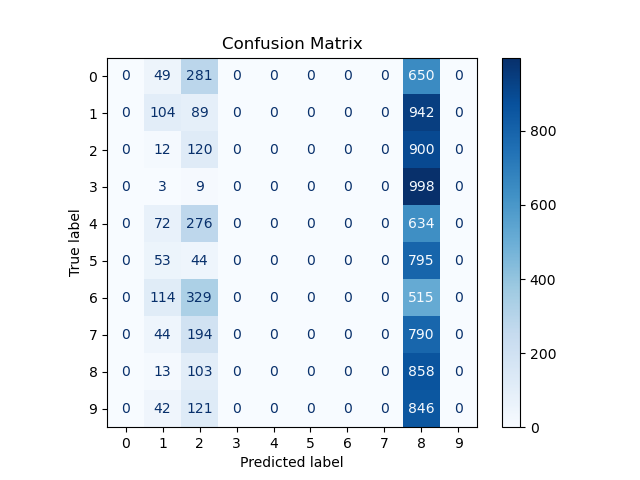
\includegraphics[width=0.80\textwidth]{Immagini/Grafici/confusion_matrix_prima.png}
    \caption{Situazione prima del training}
    \label{fig:DNN_con_matrix_prima}
\end{figure}

In sole $30$ epoche la rete neurale è riuscita ad "imparare" a classifica correttamente 
buona parte degli esempi di test.

\begin{figure}[H]
    \centering
    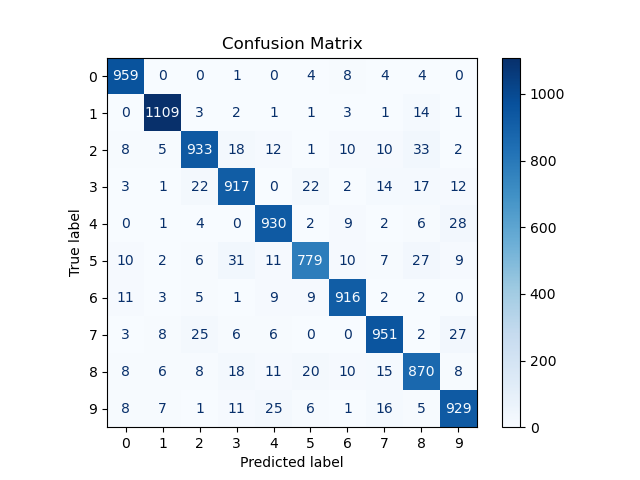
\includegraphics[width=0.80\textwidth]{Immagini/Grafici/confusion_matrix_dopo.png}
    \caption{Situazione dopo il training}
    \label{fig:DNN_con_matrix_dopo}
\end{figure}

Dall'immagine (\ref{fig:DNN_accuracy_dopo}) possiamo osservare come è migliorata la 
precisione del modello nella predizione sul dataset di validazione nel corso delle 
epoche, arrivando ad ottenere una precisione di circa del $93\%$. 
% Un valore migliorabile addestrando la rete 
% ancora per qualche epoca.  

\begin{figure}[H]
    \centering
    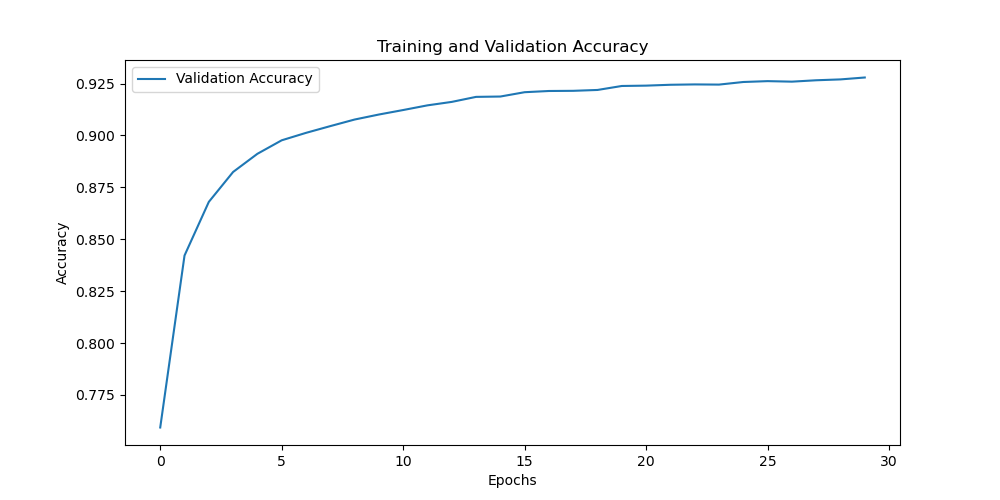
\includegraphics[width=1.0\textwidth]{Immagini/Grafici/training_validation_accuracy_v1.png}
    \caption{Andamento dell'accuratezza}
    \label{fig:DNN_accuracy_dopo}
\end{figure}

Mentre dall'immagine (\ref{fig:DNN_loss}), possiamo osserva l'andamento della loss 
durante la fase di training e validation. 

\begin{figure}[H]
    \centering
    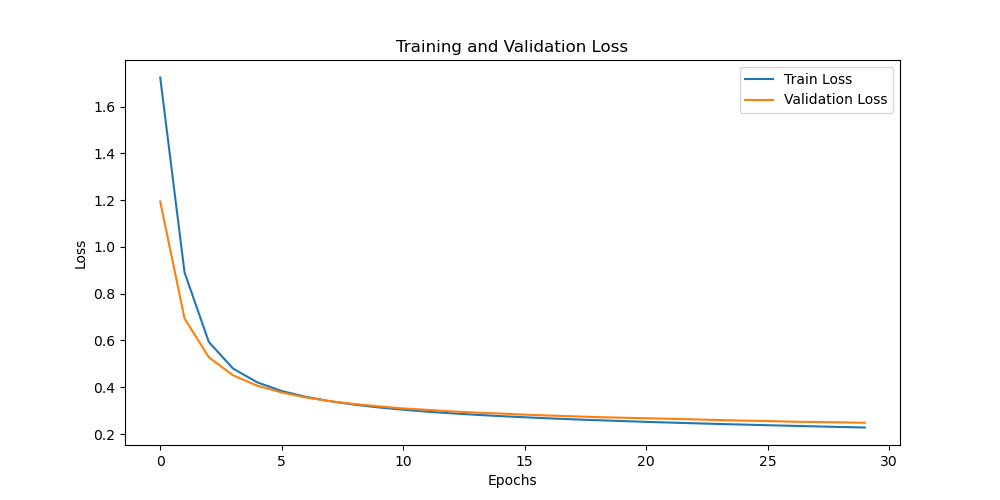
\includegraphics[width=1.0\textwidth]{Immagini/Grafici/training_validation_loss_v1.png}
    \caption{Andamento delle loss}
    \label{fig:DNN_loss}
\end{figure}

\newpage
\subsection{Limitazioni}

Come si può intuire osservando la figura (\ref{fig:MNIST_processato}), uno dei principali
problemi risiede nel fatto che queste tipologie di reti neurali non risultano essere
invarianti rispetto a traslazioni e distorsioni dell’immagine.

Ovvero che sono sensibili alle minime variazioni dell'immagine. Quindi non risultano 
essere particolarmente adatte per queste applicazioni in cui le immagini possono 
variare in tanti aspetti.

Una soluzione al problema dell’elaborazione delle immagini è stata proposta nel 1998
da Yann LeCun, il quale propose un nuovo metodo di estrazione delle features:
ogni immagine è suddivisa in diverse aree e da esse verranno estratte le caratteristiche
(features) più significative, mediante l’utilizzo di filtri. Tale intuizione ha portato alla
nascita delle reti neurali convoluzionali.

\begin{figure}[H]
    \centering
    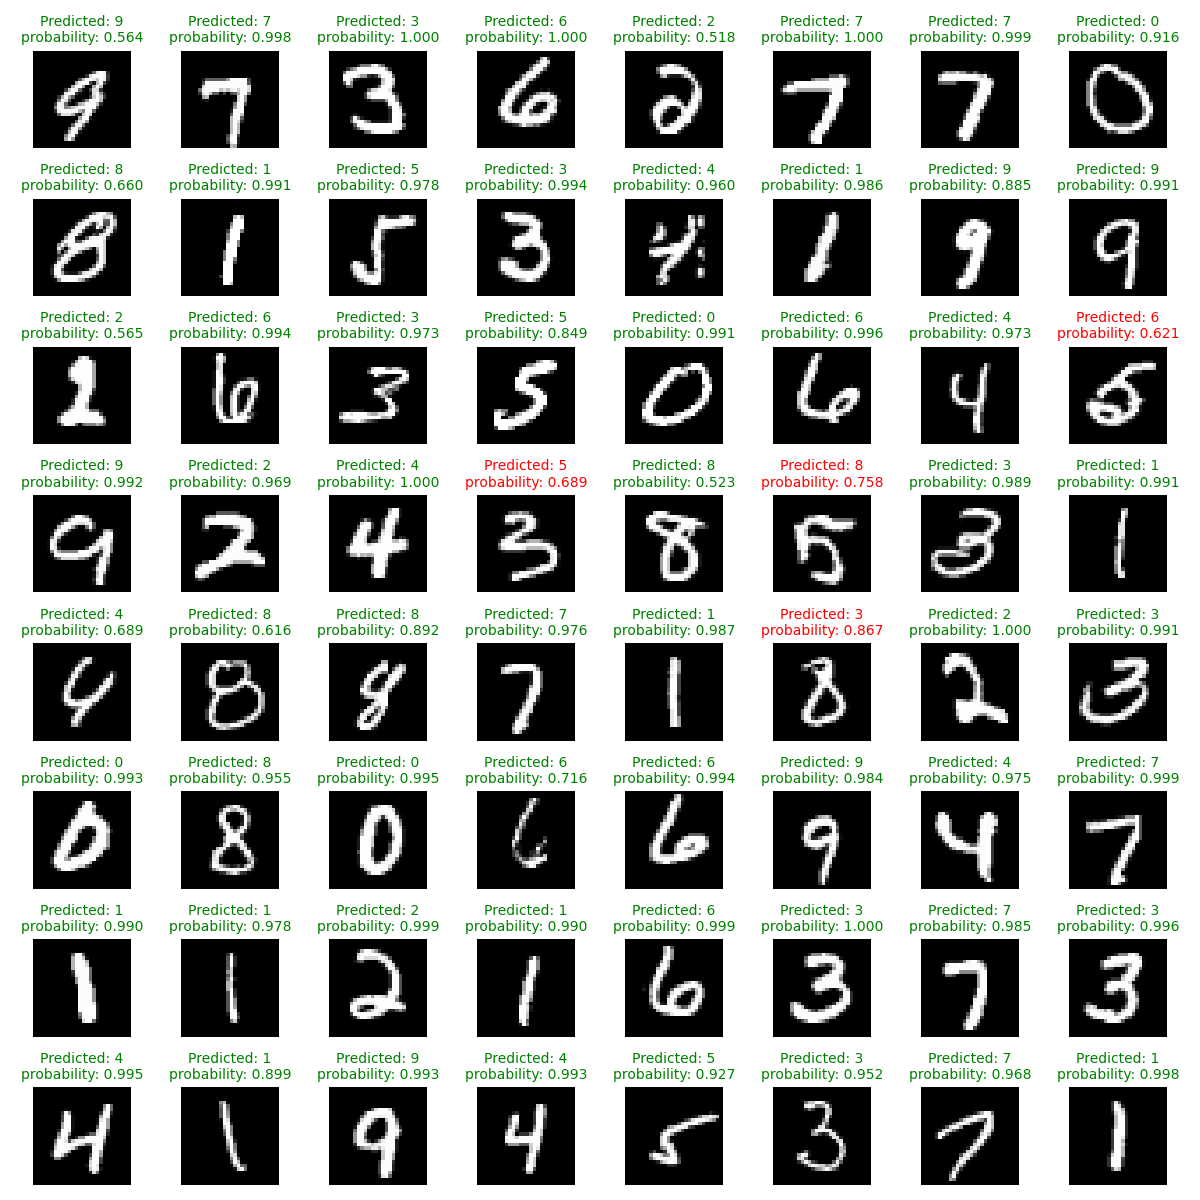
\includegraphics[width=1.0\textwidth]{Immagini/Grafici/esempio_MNIST_processato.png}
    \caption{Esempio di alcuni campioni}
    \label{fig:MNIST_processato}
\end{figure}

